\documentclass{zbc-report}

\usetikzlibrary{shapes.geometric}  % Including shapes.geometric for TikZ
\usepackage[normalem]{ulem}
\useunder{\uline}{\ul}{}

%% Set up the bibliography
\usepackage[backend=biber, style=apa]{biblatex}
\addbibresource{report.bib}

%% Additional packages and commands
\usepackage{parskip}
\setlist{itemsep=-2pt} % Reducing white space in lists slightly
\renewcommand{\deg}{\si{\degree}\xspace} % Use \deg easily, everywhere

%% Set up the minted package
\usepackage[cachedir=_minted-report]{minted}
\setminted{
    linenos=true,
    breaklines=true,
    fontsize=\footnotesize,
    frame=lines,
    framesep=2mm,
    baselinestretch=1.2,
    bgcolor=gray!10,
    style=vs,
    mathescape=true,
}

%% ----------------------------------------------------------------------
%%    Begin of document + Frontmatter (Roman page numbering)
%% ----------------------------------------------------------------------

\begin{document}

\frontmatter

%% Define the main parameters
\title{Metode sammenligning}
\subtitle{Systemudvikling \\ 3. Semester}
\author{Carsten Lydeking}

\subject{Projektprocesser} % Cover only
\large\affiliation{Zealand Business College} % Cover only
\coverimage{figures/template-figures/binary.jpg} % Aspect ratio of 2:3 (portrait) recommended
\definecolor{title}{HTML}{4884d6} % Color for cover title

\makecover

\begin{titlepage}

\begin{center}

%% Print the title
{\makeatletter
\largetitlestyle\fontsize{45}{45}\selectfont\@title
\makeatother}

%% Print the subtitle
{\makeatletter
\ifdefvoid{\@subtitle}{}{\bigskip\titlestyle\fontsize{20}{20}\selectfont\@subtitle}
\makeatother}

\bigskip
\bigskip

%% Print the name of the author
{\makeatletter
\largetitlestyle\fontsize{25}{25}\selectfont\@author
\makeatother}

\bigskip
\bigskip

%% Print table with names and student numbers
\setlength\extrarowheight{2pt}
\begin{tabular}{c}
    cal002@edu.zealand.dk \\
\end{tabular}

\vfill

%% Print some more information at the bottom
\begin{tabular}{l r}
    Lecturer, SWD:   & Michael Hammel \\
    Project Deadline: & \ddmmyydate{14/10/24} \\
    Handed-in:       & \ddmmyydate{\today} \\
    Faculty:         & Systemudvikling \\
    Semester:        & 3. Semester\\
    Word Count:      & xxxx Characters (including spaces) \\ %% Counted using texcount, not included in template
\end{tabular}

\bigskip
%% Add a source and description for the cover and optional attribution for the template
\begin{tabular}{l r}
    Cover: & Generated image of binary using DALL-E \\
    Style: & ZBC template -- created by Carsten Lydeking (Cally) \\
\end{tabular}


%% Insert the Zealand logo at the bottom of the page
\begin{tikzpicture}[remember picture]
    \node[above=10mm] at (current page.south) {%
        \includegraphics[width=0.35\textwidth]{figures/template-figures/zealandcombinedlogo}
    };
\end{tikzpicture}

\end{center}

\end{titlepage}

\tableofcontents
% \listoffigures
% \listoftables

%\input{front/nomenclature}

%% ----------------------------------------------------------------------
%%    Mainmatter (Arabic page numbering)
%% ----------------------------------------------------------------------

\mainmatter

\chapter{Intro}
\label{chapter:introduction}

\section{Formål}
\label{sec:case}
Formålet med denne opgave er at sammenligne forskellige systemudviklingsmetoder for at forstå
i hvilke konkrete sammenhænge en metode kan være gavnlig.
Hertil er det bundet, at vælge XP som den ene. Dertil er spiralmodellen valgt som den anden metode.
Why - fordi spiralmodellen, var en metode vi allerede havde fremlagt om.

\section{Om referencerne}
\label{sec:note}
Alle referencer er listet bagerst i dokumentet, i APA format. I selve dokumentet er de referet i et APA godkendt format til in-line referencer. Læser man dokumentet elektronisk kan man blot klikke på referencen og blive ført til referencen i referencelisten.

\chapter{XP}
\label{chapter:2ndchapter}
Som primært opslagsværk er bogen \cite{beck2004xp} blevet anvendt.

\textbf{Baggrund:}\\
Extreme Programming (XP) blev udviklet af Kent Beck i slutningen af 1990'erne. 
Det blev oprindeligt introduceret som en måde at forbedre softwareudviklingsprocessen i situationer, 
hvor kundens krav ofte ændrede sig. XP blev født som en reaktion på de udfordringer, 
traditionelle vandfaldsmodeller stod over for, når de skulle håndtere skiftende krav og behov for fleksibilitet.

Kent Beck begyndte at eksperimentere med XP, mens han arbejdede på et projekt for Chrysler Corporation. 
Han fokuserede på at fremme hurtig feedback, hyppig udgivelse af små funktionaliteter og tæt samarbejde mellem udviklere og kunder. 
Beck offentliggjorde først sine ideer om XP i 1999 med bogen "Extreme Programming Explained: Embrace Change." 
Modellen fik hurtigt momentum blandt agile tilhængere og blev en af de mest populære agile udviklingsmetoder.
Som en sidenote, så blev Chrysler-projektet aldrig færdiggjort - much in the spirit of Agile.. 

\textbf{Formål og fokus:}\\
XP fokuserer på at levere høj kvalitet og værdifuld software gennem hyppige iterationer, hvor koden konstant forbedres. 
Den understøtter praksisser som parprogrammering, test-drevet udvikling (TDD) og kontinuerlig integration, hvilket hjælper teams med at levere funktionalitet hurtigere og med færre fejl.
XP en af de mest ekstreme agile metoder, og den er ikke nødvendigvis egnet til alle projekter.

\textbf{Fremdrift og styring af fremdrift:}\\
XP styrer fremdriften gennem korte iterationer (cyklusser) på 1-2 uger. I hver cyklus leveres ny funktionalitet, og udviklerne samarbejder tæt med kunden. Projektet tilpasses løbende, så ændrede krav hurtigt kan implementeres, hvilket (burde) sikrer konstant fremdrift.

\textbf{Kvalitet i produktionen:}\\
Kvalitet sikres gennem teknikker som parprogrammering, test-drevet udvikling (TDD) og hyppige kodegennemgange. XP fokuserer på at opfange fejl tidligt, hvilket skulle kontinuerligt forbedrer kodekvaliteten.

\textbf{Dokumentation:}\\
Dokumentationen i XP er minimal. XP lægger vægt på at skabe forståelse gennem koden og kommunikationen i teamet, frem for at nedfælde alting skriftligt. Kun det mest nødvendige dokumenteres.

\textbf{Sikring af, at "det rigtige bliver lavet rigtigt":}\\
XP sikrer, at det rigtige produkt bliver udviklet gennem tæt samarbejde med kunden. Kunden leverer feedback i slutningen af hver iteration, så produktet konstant kan tilpasses efter deres behov.

\textbf{Vidensdeling og teamsamarbejde:}\\
Vidensdeling i XP sker gennem daglige stand-up møder og tæt samarbejde mellem teammedlemmer. Parprogrammering sikrer, at viden deles mellem udviklerne, og at ingen sidder alene med kritisk viden.

\textbf{Risikostyring:}\\
XP håndterer risici ved at bryde arbejdet op i små iterationer, så ændringer kan imødekommes hurtigt. På grund af den korte feedback-cyklus kan problemer løses tidligt, men risikostyring er ikke formelt struktureret som i andre metoder.

\textbf{Budget og tidsstyring:}\\
XP prioriterer hurtig levering af funktionalitet, hvilket kan give god kontrol over budgettet, da man kan justere omfanget af funktioner undervejs. Den fleksible tilgang kan dog skabe risiko for budgetoverskridelser, hvis omfanget ikke kontrolleres.

\chapter{Spiralmodellen}
\label{chapter:3rdchapter}
Som primært opslagsværk er artiklen \cite{boehm1988spiral} blevet anvendt. 

\textbf{Baggrund:}\\
Spiralmodellen blev introduceret af Barry Boehm i 1988 i hans artikel "A Spiral Model of Software Development and Enhancement." - som også er anvendt som primær kilde. 
Boehm udviklede Spiralmodellen som et forsøg på at kombinere styrkerne fra både vandfaldsmodellen og den iterative udviklingsmodel, 
samtidig med at han adresserede de mangler, som traditionel softwareudvikling havde, når det kom til risikohåndtering.

Spiralmodellen blev populær i store og komplekse softwareprojekter, især i miljøer med høj risiko, 
såsom forsvars- og rumfartsindustrien. Modellen tilbyder en ramme, hvor risikostyring er centralt for hver udviklingsfase, 
hvilket hjælper teams med at navigere igennem komplekse problemstillinger og reducere sandsynligheden for dyre fejl senere i processen.
Det fornemmes klart på modellen, at det er en meget pseudovidenskabelig tilgang til softwareudvikling. 
Blandet andet anvendes begreber som det angulære moment i spiralen, som et udtryk for fremdrift - Hvis et burndown chart er en DJØF'ers våde drøm, så må det være ingeniørens ditto.

\textbf{Formål og fokus:}\\
Spiralmodellen har sit fokus på risikostyring. Hver iteration, eller "spiral," begynder med en analyse af risici, 
hvorefter der træffes beslutninger om, hvordan udviklingsarbejdet skal fortsætte. Modellen giver en fleksibilitet, 
som gør det muligt at gå tilbage og revurdere tidligere beslutninger, hvilket gør den ideel til projekter, hvor kravene kan ændre sig eller er ukendte fra starten.

\textbf{Fremdrift og styring af fremdrift:}\\
I Spiralmodellen er fremdriften organiseret i faser, hvor hver iteration repræsenterer en udviklingscyklus, der slutter med en leverance. 
Hver cyklus starter med en planlægningsfase, hvor risici vurderes, og projektet evalueres, før det bevæger sig videre til næste iteration.

\textbf{Kvalitet i produktionen:}\\
Kvaliteten sikres gennem den iterative proces, hvor produktet konstant vurderes og forbedres i hver spiral. 
Den regelmæssige evaluering af både risici og funktionalitet medvirker til, at man undgår store fejl, og at der er løbende fokus på kvalitet.

\textbf{Dokumentation:}\\
Spiralmodellen lægger vægt på grundig dokumentation i hver fase af projektet. 
Dette sikrer, at både risikovurderinger, tekniske beslutninger og projektets fremgang er veldokumenteret, hvilket gør modellen velegnet til projekter med krav om formel dokumentation.

\textbf{Sikring af, at "det rigtige bliver lavet rigtigt":}\\
Spiralmodellen sikrer, at det rigtige produkt udvikles gennem løbende evaluering af både krav og risici i hver iteration. 
Ved afslutningen af hver cyklus revurderes projektet, og der tages beslutninger om, hvordan udviklingen skal fortsætte.

\textbf{Vidensdeling og teamsamarbejde:}\\
Spiralmodellen har mindre fokus på daglig vidensdeling sammenlignet med XP, men sikrer, 
at alle teammedlemmer er opdaterede gennem den formaliserede planlægnings- og dokumentationsproces, der findes i hver fase.

\textbf{Risikostyring:}\\
Risikostyring er et centralt element i Spiralmodellen. Hver iteration starter med en grundig risikovurdering, 
som styrer beslutningerne for den kommende fase. Det gør modellen særligt velegnet til komplekse projekter med stor usikkerhed.

\textbf{Budget og tidsstyring:}\\
Spiralmodellen håndterer budget og tidsstyring gennem detaljeret planlægning i hver fase. 
Den formaliserede struktur med klare milepæle og risikostyring gør det lettere at kontrollere budgettet og overholde tidsplanen sammenlignet med mere fleksible metoder som XP.

\chapter{Sammenligning}
\label{chapter:conclusion}
Dette afsnit er en sammenfatning af de foregående kapitler og indeholder mine egne konklusioner.



\section{XP og Spiralmodellen}
XP er en agil metode, der egner sig bedst til projekter med hyppige ændringer, hvor tæt samarbejde med kunden og hurtig levering er centralt. 
Spiralmodellen er bedre egnet til komplekse og risikofyldte projekter, hvor formel dokumentation, risikostyring og planlægning er nødvendigt.

\section{Spiderchart af XP og Spiralmodellen}
\label{sec:spiderchart}
\begin{figure}[H]
    \centering
    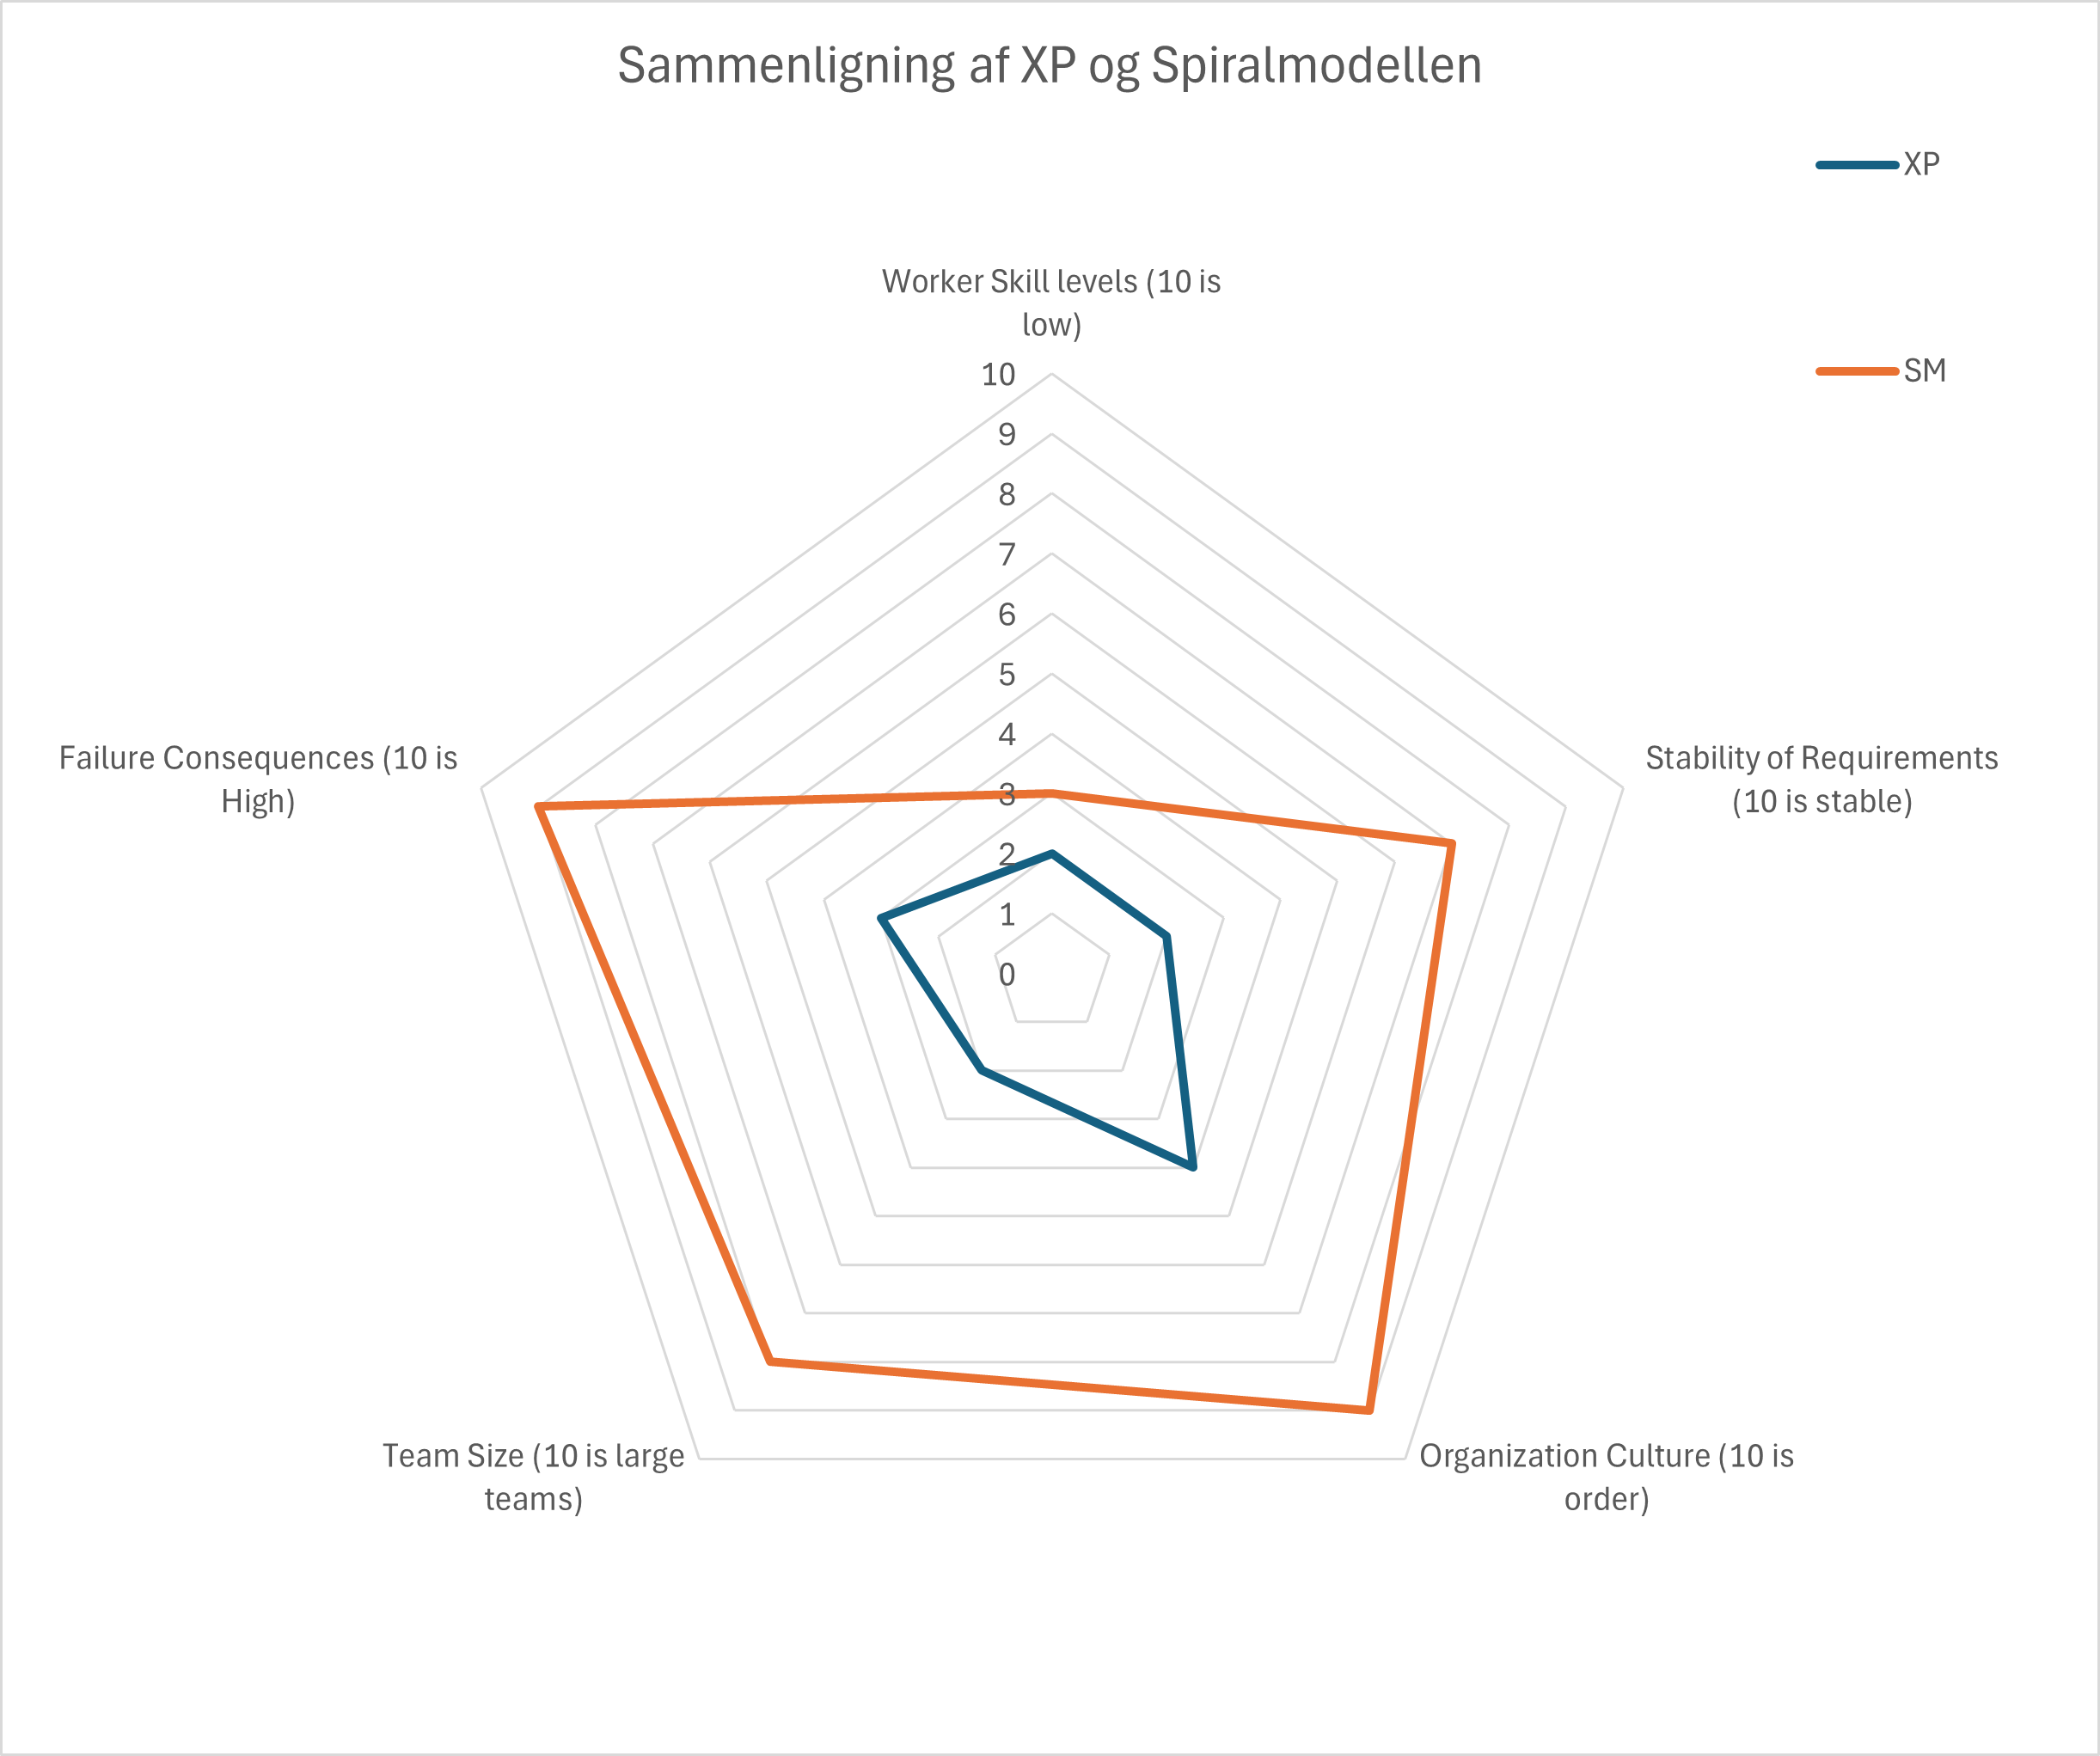
\includegraphics[width=0.8\textwidth]{figures/spiderchart.png}
    \caption{Sammenligning af XP og Spiralmodellen}
    \label{fig:spiderchart}
\end{figure}

\textbf{Skriv noget klogt om diagrammet:}\\
Diagrammet viser en sammenligning af XP og Spiralmodellen på fem parametre
\begin{itemize}
    \item Worker Skill Level - Hvor dygtige skal medarbejderne være, 1 repræsenterer her høj kompetence.
    \item Stability of requirements - Hvor ofte ændres kravene, 10 repræsenterer her stabile krav.
    \item Organizations culture - Hvor tilpasningsdygtig er organisationens medarbejderne, 10 repræsenterer formel struktur og stort behov for orden.
    \item Team Size - Hvor stort er teamet, 10 repræsenterer her et stort team.
    \item Failure Consequences - Hvor store er konsekvenserne af fejl, 10 repræsenterer her katastrofale konsekvenser.
\end{itemize}
XP og Spiralmodellen scorer lavt på Worker Skill Level, da de begge kræver medarbejder med højt kompetenceniveau. 
XP scorer lavt på Stability of requirements, Organizations culture, Team Size og Failure Consequences, mens Spiralmodellen her scorer højt.

\section{Konklusion - nu med syv tommer søm}
Valget mellem de to metoder afhænger af projektets karakter: XP er velegnet til små, fleksible projekter, mens Spiralmodellen er bedre til større projekter med mange usikkerheder og stor risiko for katastrofe ved fejl.

\section{Disclaimer}
Jeg har forsøgt, at være så objektiv som mulig, men jeg skal også klart indrømme, at jeg har stærke personlige holdninger.
Jeg har derfor nedfældet mine egne holdninger i det følgende underafsnit, så eventuelle svipsere i det skrevne hastigt kan henvises til dette afsnit som en slags fejlkilder.

\subsection{Egne holdninger}
Plan-drevet udvikling er som økonomisk videnskab - Det ligner sund matematik indtil man opdager at hele baduljen er hængt op på tesen om, at mennesket handler rationelt.
Herefter er det en lang række af modsatrettede forudsigelser, baseret på esoteriske modeller (gerne noget avanceret matematik, så chefen ikke spørg for meget) og derefter en masse undskyldninger for hvorfor det gik galt. 
Det var jo fordi, der ikke var taget højde for \textit{insert random faktor} i sine requirements, kunden er dum og kaffen smagte forkert den torsdag.
Det virker dog også altid at fortælle chefen, at det er fordi "det er en kompleks verden" - det er jo ikke forkert. 
\\
Agile er som kommunisme - Skabt af teoretikkere uden det store held indenfor eget felt, som en desperat kritik af det bestående.
Herefter revolutionært implementeret i falerede stater/organisationer under stærk propaganda af mennesker med egne agendaer. 
Når katastroferne så hobber sig op, så er det altid fordi "det var ikke ægte agile".
Herefter skal projektet bruge flere penge på at blive mere agilt, indhente flere konsulenter og så er cirklen sluttet.
Forskellene mellem XP, KANBAN og SCRUM, er i øvrigt de sammen som forskellene mellem Stalinisme, Leninisme og Marxisme. 
\\
Gid softwareudvikling var så simpelt som at skrive en bog.

%% Prevent urls running into margins in bibliography
\setcounter{biburlnumpenalty}{7000}
\setcounter{biburllcpenalty}{7000}
\setcounter{biburlucpenalty}{7000}

%% Add bibliography
\printbibliography[heading=bibintoc,title={References}]

%% ----------------------------------------------------------------------
%%    Appendix (Letters for chapters)
%% ----------------------------------------------------------------------

\appendix

% \input{appendix/appendix-sourcecode.tex}
% \input{appendix/appendix-diagrams.tex}

\end{document}